% !TeX root = ../main.tex
% !TeX spelling = EN_gb


\chapter{Introduction}\label{ch:intro} 

%https://www.iarc.who.int/infographics/global-burden-of-cutaneous-melanoma-in-2020-and-projections-to-2040/
Skin cancer is one of the most widespread and fatal cancer types globally \cite{karimkhani2017global}. It generally develops due to exposure to ultraviolet (UV) rays from the sun, which harms the DNA of skin cells. Some artificial sources of light, in particular tanning beds and sunlamps, increase the risk of developing this disease \cite{narayanan2010ultraviolet}. In 2022, an estimated 99,780 adults (57,180 men and 42,600 women) in the United States will have been diagnosed with invasive melanoma of the skin \cite{co2022american}. Worldwide, there approximately 324,635 people were newly diagnosed with melanoma in 2020 and 57,000 people died from the disease. A new study by scientists from the International Agency for Research on Cancer (IARC) and partners predicts that the number of new cases of cutaneous melanoma per year will increase by more than 50$\%$ from 2020 to 2040  \cite{world2022international}, as shown in Figure \ref{Fig:Mel1}. 

\begin{figure}
\centerline{
 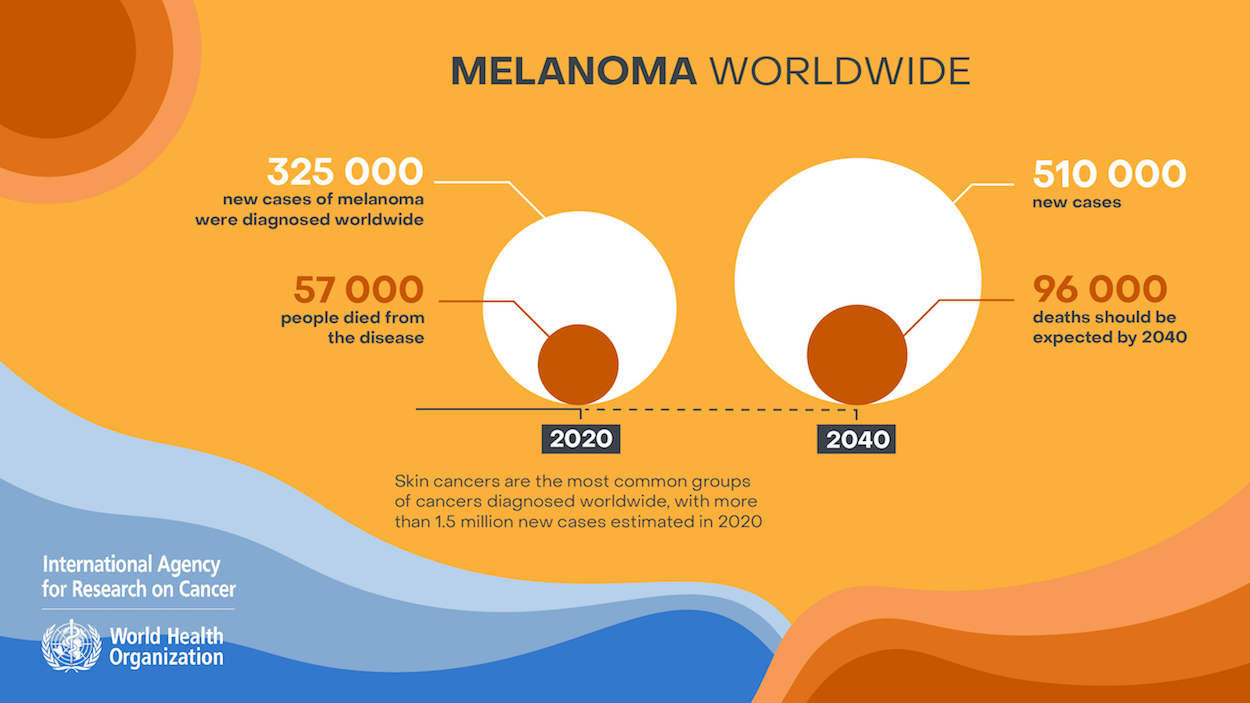
\includegraphics[width=\linewidth]{Melanoma_infog_1} 
 }
\caption{Dermatology statistics in 2020 and forecast for 2040\cite{world2022international}.}
\label{Fig:Mel1}
\end{figure}

% Di Leo, et al. \cite{di2015web} showed that expert dermatologist has been revealed as the best (94$\%$), whereas the automatic system alone has shown a satisfying accuracy of 79$\%$. non-expert
% dermatologist greatly beneficiated from automatic system assistance (presentations of both the results corresponding to single criterion detection and lesion classification) during dermoscopic images
% evaluation, with an improvement in diagnostic sensitivity (from
% 68$\%$ to 90$\%$) without compromising specificity (also improved
% from 84$\%$ to 92$\%$) and resulting in a significant gain in terms
% of diagnostic accuracy (from 80$\%$ to 92$\%$). The statistics from  Di Leo, et al.\cite{di2015web} suggest that automation can help early-stage dermatologists improve diagnostic performance. Maybe in the future, it will not replace the position of the doctor's diagnosis, but it can assist the medical system to be more effective. This reason is sufficient to justify the need for computer-aided diagnosis (CAD) systems for skin cancer.
Di Leo, et al. \cite{di2015web} compiled Table \ref{comp}, which compares the performances of the expert dermatologists, non-expert dermatologists, and automatic measurement systems. This table shows that non-expert dermatologists greatly benefit from automatic system assistance (concerning results corresponding to single-criterion detection and lesion classification) during dermoscopic images evaluation, with an improvement in diagnostic sensitivity (from 68$\%$ to 90$\%$) without compromising specificity (which also improved from 84$\%$ to 92$\%$) and resulting in a significant gain in terms of diagnostic accuracy (from 80$\%$ to 92$\%$). Computer-aided diagnosis (CAD) systems can help the medical system to be more effective.

\begin{table}[!htbp]
\centering
\caption{Performance comparison \cite{di2015web}.}\label{comp}
\scalebox{0.7}{
\begin{tabular}{p{7cm}ccc}
\hline
\textbf{Analysis type} &\textbf{Sensitivity}($\%$) &\textbf{Specificity}($\%$) & \textbf{Accuracy}($\%$)\\
\hline
Expert dermatologist (ED)& 92& 95 &94\\
\hline
Automatic measurement systems (MS)& 90& 75&79 \\
\hline
Non-expert dermatologist (NED)& 68& 84&80 \\
\hline
NED + MS& 90& 92&92 \\
\hline
\end{tabular}
}
\end{table}






Skin cancer,  the most common type of cancer that affects humans, is usually diagnosed by initial clinical screening, which is followed by dermoscopic analysis. Dermoscopy can effectively allows the visualization of subsurface structures of the skin, revealing lesion details in colors and textures not normally visible to the naked eye \cite{argenziano2001dermoscopy}. It is widely used in skin lesion diagnostic systems and has become a vital assistant technology for dermatologists. 

 Automatic skin lesion classification in dermoscopy images is an essential task of CAD \cite{tang2020gp}. With the help of the fast development of image processing and artificial intelligence (AI) algorithms for disease diagnosis and prognostication, the chances of surviving many forms of cancer have been increasing considerably in recent years \cite{iqbal2021automated}.  Due to the increased demands that skin cancer cases are imposing on global healthcare services, the need for remote automated diagnostic solutions is becoming increasingly pressing \cite{cassidy2022analysis}. This is especially pertinent in poorer countries where patients do not have access to the latest medical equipment and expertise required for accurate diagnosis. For example, in emerging countries such as Brazil, there is a notable lack of dermatologists and dermatoscopes in most small cities \cite{pacheco2020impact}. 
 
 In recent decades, skin lesion classification has become a popular field of research following the growing adoption of machine-learning techniques in the field of medical image analysis. Pioneering works, such as \cite{umbaugh1993automatic,ercal1994neural,green1994computer} have reported the use of low-level handcrafted features to differentiate melanomas and keratinocyte cancers. Later, different computational approaches have been developed based on the ABCD(E) rule \cite{rigel2005abcde}, pattern analysis, and seven-point checklist \cite{di2010automatic}, which are common methods used by dermatologists to diagnose skin cancer. These approaches mostly use traditional computer vision algorithms to extract various features such as shape, color, and texture to feed a classifier. However, the handcrafted features extracted by these methods have limited generalizability \cite{yu2016automated}.

\begin{figure}[!h]
\centering
	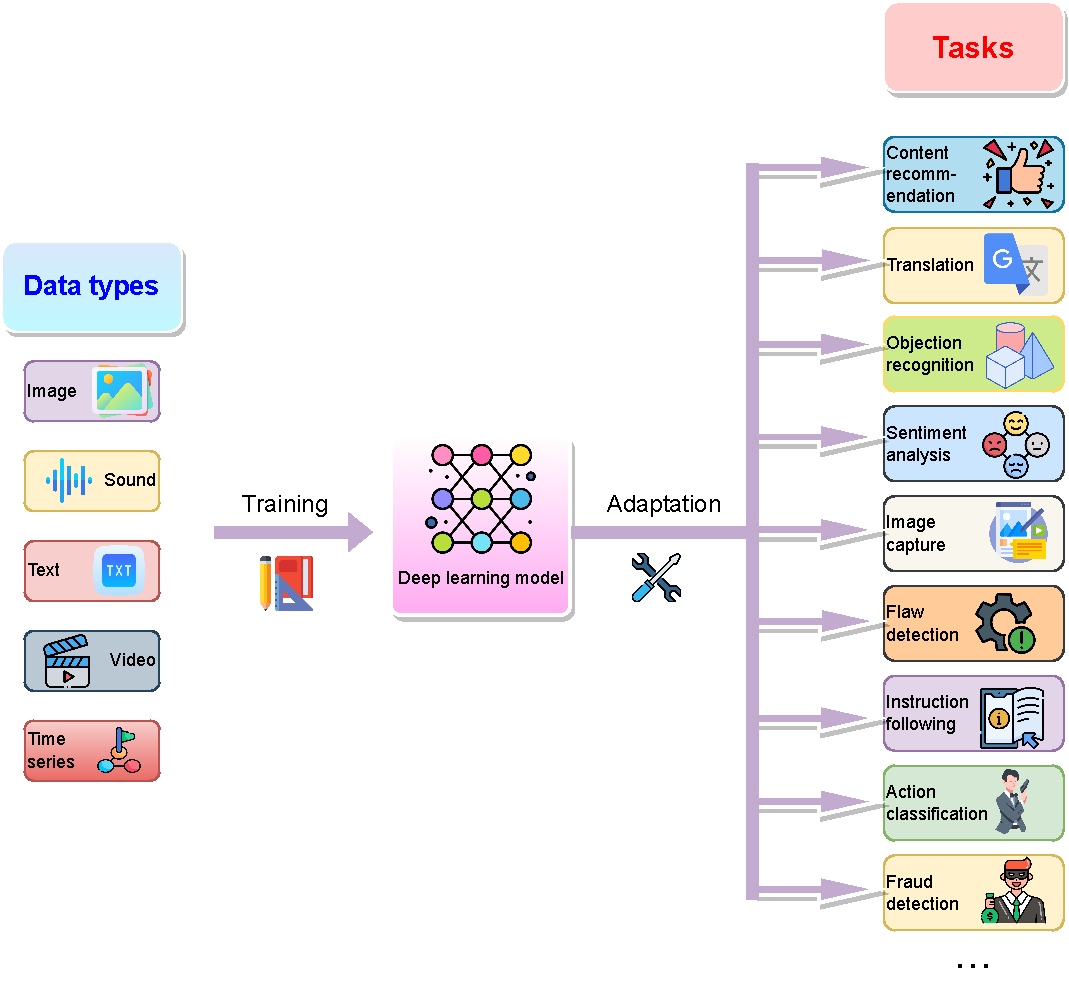
\includegraphics[width=4.5in]{tasks}
		\caption{A deep learning model can centralize the information from all the data from various modalities. This one model can then be adapted to a wide range of downstream tasks.}
		\label{Fig:tasks} 
\end{figure}
 
Deep learning models are good at identifying patterns in unstructured data, and in most  media data such as images, sounds, texts, videos, and time series. Figure \ref{Fig:tasks} above shows the types of applications. Recently, deep learning models have been also achieving remarkable results in various medical image analysis tasks \cite{yu2016automated,lin2020comparison,eskandari2022frailty,azeem2021covid,romo2020end}. Esteva et al. \cite{esteva2017dermatologist} have demonstrated the dermatologist-level classification of skin cancer by deep learning. They used 129,450 images to train and ultimately validate a system using binary classes (benign/malignant). The performance of the classification method used in the CNN system by Esteva et al. \cite{esteva2017dermatologist} was on par with that of all of the dermatologists who participated. Brinker et al. \cite{brinker2019deep} proved that CNN outperformed 136 of 157 dermatologists in a head-to-head dermoscopic melanoma image classification task as shown in Figure \ref{Fig:CNNP}. 

%\cite{brinker2019deep}
In this thesis, I focus on deep learning approaches to skin lesion classification using
dermoscopic images.

\begin{figure}[!h]
\centering
	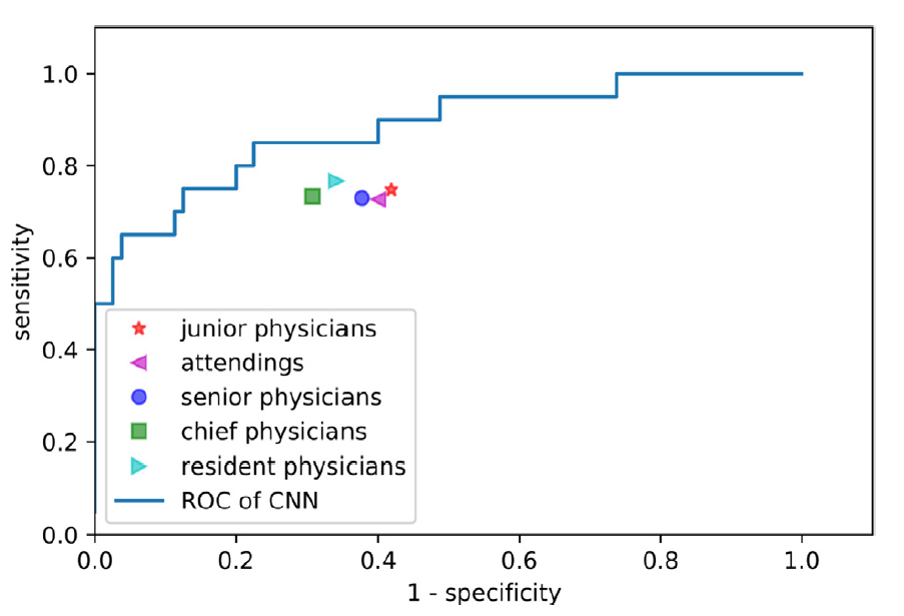
\includegraphics[width=4.5in]{AvP}
		\caption{The average performance of physicians from all hierarchical levels within dermatology (from junior to chief) and CNN \cite{brinker2019deep}.}
		\label{Fig:CNNP} 
\end{figure}



\section{Problem formulation/motivation}
%%% node design and implementation
 The automated classification of skin lesions is still a challenging task because of the great visual similarity between melanoma and benign lesions \cite{hosny2022refined}. The first problems are the intra-class differences and inter-class similarities of skin lesions, which cause many difficulties in the identification of malignant and benign skin lesions. Since variation in the appearances of skin lesions  is small, local, and subtle, fine-grained global context information is essential for skin lesion recognition.                                                                                     

% Motivated by these three main questions of dermatological classification we carried out this research project.
Skin cancer is on the rise without a corresponding increase in the number of dermatologists. The good news is that diagnosis of skin diseases plus CAD can greatly assist non-expert diagnosis. Medical diagnosis in remote areas is becoming increasingly urgent, so remote diagnosis will also become a trend. Deep learning methods have also grown dramatically in the field of dermatology in recent years, but most of them are based on large volumes of data. However, collecting high-quality medical images is not easy in hospitals, and gaining research approval of applications for research is even more difficult. I initially targeted small datasets; over time, I eventually targeted large data sets and multiple classifications, where the extreme imbalance of data also affects the accuracy of classification. Improving the accuracy of skin disease classification is an endless pursuit. All the above-mentioned considerations motivated us to carry out this research project.



\section{Research objectives} \label{sec.questions}

The aim of this project is to construct a deep convolution neural network to automatically examine and classify skin lesions using dermoscopic images. By being able to early filter out, at an early stage, patients who do not need to see a doctor, the goal is to reduce the burden put on the doctors to allow more people to be checked
regularly.  The goal is to achieve a high enough classification accuracy. This leads to the following four research questions (RQs) and associated contributions:

\subsection{Literature review}
I conducted a literature review alongside our in-depth study of the chosen problem. I found a considerable amount of previous work, showing that the use of CAD to classify skin diseases is not a new research topic.  
\begin{itemize} \label{sec.rq1}
    \item \textbf{RQ1.} Does the research on automated melanoma detection contain aggregated knowledge and structures?
\end{itemize}

\subsubsection{Paper \uppercase\expandafter{\romannumeral5} (review paper):} This paper addresses \textbf{RQ1}.

%\subsubsection{\textit{Contribution:}}

\textit{Contribution: }
In this literature review, I selected more than 200 high-quality papers for analysis and research. The purposes of this review were to: understand the most state-of-art deep learning methods for dermatology classification; understand the most commonly used research methods, model frameworks, and data used; identify the challenges and unsolved problems still facing the field of dermatology research; and identify ideas for future research. I also found that most of the deep learning methods simply  just aggregate different CNN backbones to conduct skin cancer classification.
  
\subsection{Small dataset}
Another problem is the poor generalization ability of the deep convolutional neural network (DCNN) under training with a limited skin lesion dataset. Therefore, how to effectively classify skin cancer when using small databases is another challenge.
\begin{itemize} \label{sec.rq2}
    \item \textbf{RQ2.} Can a small dataset yield good experimental results in skin cancer classification based on deep learning?   
\end{itemize}

\subsubsection{Papers \uppercase\expandafter{\romannumeral1} (Yolo) $\&$  \uppercase\expandafter{\romannumeral2} (k-fold):}
These two papers address \textbf{RQ2}.

%\subsubsection{\textbf{Contribution:}}
\textit{Contribution: }
Due to the limitations of hardware resources and the difficulty of collecting medical images, I initially used small dataset images for our research. Both of these papers are based on small datasets. I chose to use the Yolo framework \cite{redmon2016you} and k-fold validation to train with small datasets while maintaining good accuracy.


\subsection{Imbalance dataset}

In addition, having imbalanced labels is a peculiarity of skin cancer datasets. The class imbalance has been shown to significantly impact model performance.

\begin{itemize} \label{sec.rq3}
    \item \textbf{RQ3.} How should the data imbalance be handled when there are many categories? 
\end{itemize}

\subsubsection {Paper \uppercase\expandafter{\romannumeral6} (hybrid+FL):}
This paper addresses \textbf{RQ3}. 

%\subsubsection{\textbf{Contribution:}}
\textit{Contribution: }
To solve the problem of data imbalance problem, three different loss functions were used and compared in this paper to adjust the weights of different skin diseases in model training. The verification produced good results. 


\subsection{Improve accuracy}
 The automated classification of skin lesions is still a challenging task because of the great visual similarity between melanoma and benign lesions \cite{hosny2022refined}. The intra-class differences and inter-class similarities of skin lesions create many difficulties in the identification of malignant and benign skin lesions. Since the variation in the appearance of skin lesions is small, local, and subtle, fine-grained global context information is important 
 for skin lesion classification.                                                                                     
\begin{itemize} \label{sec.rq4}
    \item \textbf{RQ4.} How can the accuracy of skin disease diagnosis be improved? 
\end{itemize}

\subsubsection {Papers \uppercase\expandafter{\romannumeral3} (seven-point), \uppercase\expandafter{\romannumeral4} (Cosine), $\&$ \uppercase\expandafter{\romannumeral6} (hybrid+FL):}
These address \textbf{RQ4}. 

%\subsubsection{\textbf{Contribution:}}
\textit{Contribution: }
No matter what challenge I want to solve in dermatology, the ultimate problem I face is improving the accuracy of dermatology classification. I combined the traditional machine learning method, i.e., the 7-point checklist algorithm,  with deep learning and also used different learning rates to improve model training. Finally, I applied a hybrid model, combining CNN and transformer depth model algorithms to improve classification accuracy.


\section{Dissertation outline}
The remaining chapters are organized as follows.
\begin{itemize}
  \item Chapter \ref{ch:theory} is mainly about the theoretical basis of deep learning, data sources, and use of skin disease classification; it then briefly summarizes the models and methods used.
  \item Chapter \ref{ch:method} summarizes how the published papers support the dissertation, briefly describing the present author's contribution.
  \item Chapter \ref{ch:results} explains and discusses the research findings in relation to the research objectives. It discusses the strengths and weaknesses of our research, and the trend and direction of future research on skin disease classification.
  \item Chapter \ref{ch:conclusion} summarizes the conclusions of this work and the next steps forward to take in future work.
\end{itemize}
   


\section{Contributions}
The following table presents the authors' contributions to each publication included in this thesis:\\
Y. N. - Yali Nie\\
P. S. - Paolo Sommella\\
M. C. - Marco Carratù\\
C. L. - Consolatina Liguori\\
M. F. - Matteo Ferro\\
L. D. S. - Laura De Santis\\
S. C. - Sara Cacciapuoti\\
G. D. - Giuseppe Di Leo\\
G. F. - Gabriella Fabbrocini\\
A. U. M. - Avoci Ugwiri Moise\\
M. O. - Mattias O'Nils\\
J. L. - Jan Lundgren


\begin{sidewaystable}[htbp]
  \centering
  %
  %\scalebox{0.6}{
  %\begin{threeparttable}[b]
  \caption{The list of authors' contributions to each paper(M=main contributor, C=co-author).\label{table1}}
    %\begin{tabular}{p{5.665em}cp{20.22em}p{10.28em}}
    %\resizebox{\linewidth}{!}{
    \scalebox{0.8}{
    \begin{tabular}{c c c c c c c c c c c c c p{5cm}<{\centering}}
    \midrule
    \midrule
    \multirow{2}{*}{\textbf{Paper}} & \multicolumn{12}{c}{\textbf{Authors}} & \multirow{2}{*}{\textbf{Y. N. :
    Contribution}}\\ \cline{2-13}
     & \textbf{Y. N.} 
    & \multicolumn{1}{c}{\textbf{P. S.}} 
    & \multicolumn{1}{c}{\textbf{M. C. }}
    & \multicolumn{1}{c}{\textbf{C. L. }} &\multicolumn{1}{c}{\textbf{M. F. }}
    &\multicolumn{1}{c}{\textbf{L. D. S. }}
    &\multicolumn{1}{c}{\textbf{S. C. }}
    &\multicolumn{1}{c}{\textbf{G. D. }}
    &\multicolumn{1}{c}{\textbf{G. F. }}
    &\multicolumn{1}{c}{\textbf{A. U. M. }}
    &\multicolumn{1}{c}{\textbf{M. O. }} &\multicolumn{1}{c}{\textbf{J. L. }} & \\
    \midrule
    I & M     &  C  &  & C & & & & & & &C &C&  Conceptualization, methodology, data curation, writing $\&$ editing  \\
    \hdashline[0.8pt/2pt]
    II & M     & C &  C&  & &C & & & & &C &C & Conceptualization, validation, formal analysis, writing $\&$ editing, visualization\\
    \hdashline[0.8pt/2pt]
    III & M     & C & C&  & M& &C &C &C & & &C &Investigation, resources, writing – original draft preparation\\
    \hdashline[0.8pt/2pt]
    IV & M     &C &  C&  & & & & & & C&C &C &Conceptualization, methodology, software, validation, data curation, writing $\&$ editing, visualization\\
    \hdashline[0.8pt/2pt]
    V & M     &C & C&  & C& & & & & &C &C& Conceptualization, methodology, software, formal analysis, investigation, resources, data curation, visualization, writing $\&$ editing\\
    \hdashline[0.8pt/2pt]
    VI & M     &C & C&  & & & & & & &C &C&Conceptualization, methodology, validation, formal analysis, writing $\&$ editing, visualization\\
    %\bottomrule
    \bottomrule
    \end{tabular}%
    }
 
  
  
\end{sidewaystable}%



